\documentclass[letter,12pt,sffamily]{article}
\usepackage{datetime}
\usepackage{tikz}
\usepackage{algorithm}
\usepackage{amsmath}
\usepackage[noend]{algpseudocode}
\usepackage{fontspec}
\usepackage{minted}
\usemintedstyle[c]{tango}
\usepackage{listings}
\usetikzlibrary{trees}
\makeatletter
\def\BState{\State\hskip-\ALG@thistlm}
\makeatother

\begin{document}
\tikzstyle{every node}=[thick,anchor=west, rounded corners, font={\scriptsize\ttfamily}, inner sep=2.5pt]
\tikzstyle{selected}=[draw=blue,fill=blue!10]
\tikzstyle{root}=[selected, fill=blue!30]

\begin{titlepage}
  \begin{center}
    \vspace*{1cm}
    \Huge
    \textbf{Chapter 6}\\
    \vspace{0.5cm}
    \LARGE
    Pipes and the Client-Server Model
    \vfill
    \Large
    \textbf{Jonathan Reyna}\\
    College of Engineering and Computing\\
    Nova Southeastern University\\
    \usdate{\today}
  \end{center}
\end{titlepage}

\section{Program 6.7: pipeserver}
pipeserver demonstrates a simple use case of a pipe, while embracing the client-server model. The pipe listens, just as a server would, for data written to the pipe. As data is written to the pipe, it is forwarded to the standard output file descriptor. That output is then redirected to a log file for later examination.
\subsection{Relation to Learned Material}
Chapter 6 discusses the various UNIX special files, and their practial uses in applications. It also introduces the client-server model. Program 6.7 combines these concepts. 
\subsection{Source Code}
\renewcommand{\theFancyVerbLine}{
\sffamily\textcolor[rgb]{0.5,0.5,0.5}{\scriptsize\arabic{FancyVerbLine}}}

\begin{minted}[mathescape,
    linenos,
    numbersep=5pt,
    gobble=0,
    frame=lines,
  framesep=2mm]{c}

#include <errno.h>
#include <fcntl.h>
#include <stdio.h>
#include <unistd.h>
#include <sys/stat.h>
#include "../restart/restart.h"

#define FIFOARG 1
#define FIFO_PERMS (S_IRWXU | S_IWGRP | S_IWOTH)

int main(int argc, char *argv[]) {
  int requestfd;

  /* name of server fifo is passed on the command line */
  if (argc != 2) { 
    fprintf(stderr, "Usage: %s fifoname > logfile\n", argv[0]);
    return 1;
  }
	
  /* int mkfifo(const char *pathname, mode_t mode); */
  /* Create a new FIFO named PATH,                  */ 
  /* with permission bits MODE.                     */
  if ((mkfifo(argv[FIFOARG], FIFO_PERMS) == -1) && 
      (errno != EEXIST)) {
    perror("Server failed to create a FIFO");
    return 1;
  }
	
  /* open a read/write communication endpoint to the pipe */
  if ((requestfd = open(argv[FIFOARG], O_RDWR)) == -1) {
    perror("Server failed to open its FIFO");
    return 1;
  }
  copyfile(requestfd, STDOUT_FILENO);
  return 1;
}
\end{minted}
\subsection{Environment}
\begin{figure}[H]
	\centering
	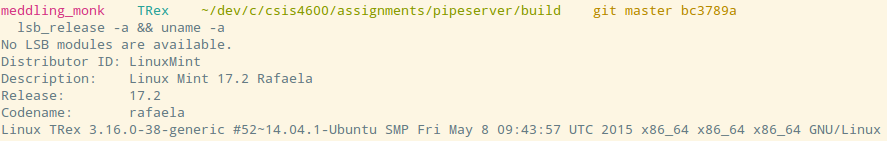
\includegraphics[width=1\linewidth]{./images/0}
	\caption[env]{Build Environment}
	\label{fig:0}
\end{figure}
\subsection{Build}
\begin{figure}[H]
	\centering
	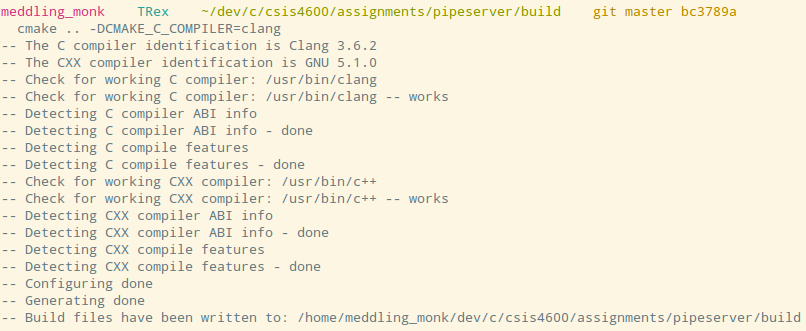
\includegraphics[width=1\linewidth]{./images/1}
	\caption[CMake_prep]{CMake Metabuild}
	\label{fig:1}
\end{figure}
\begin{figure}[H]
	\centering
	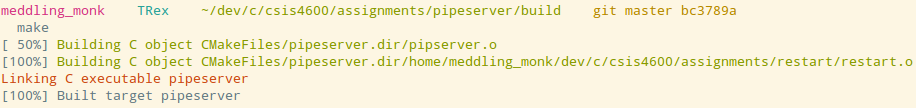
\includegraphics[width=1\linewidth]{./images/2}
	\caption[make_build]{UNIX make}
	\label{fig:2}
\end{figure}
\subsection{Run}
\begin{figure}[H]
	\centering
	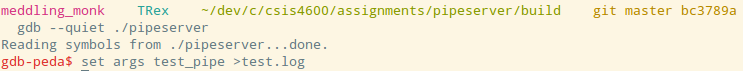
\includegraphics[width=1\linewidth]{./images/3}
	\caption[starting_GDB]{GNU Project Debugger initialization}
	\label{fig:3}
\end{figure}
\begin{figure}[H]
	\centering
	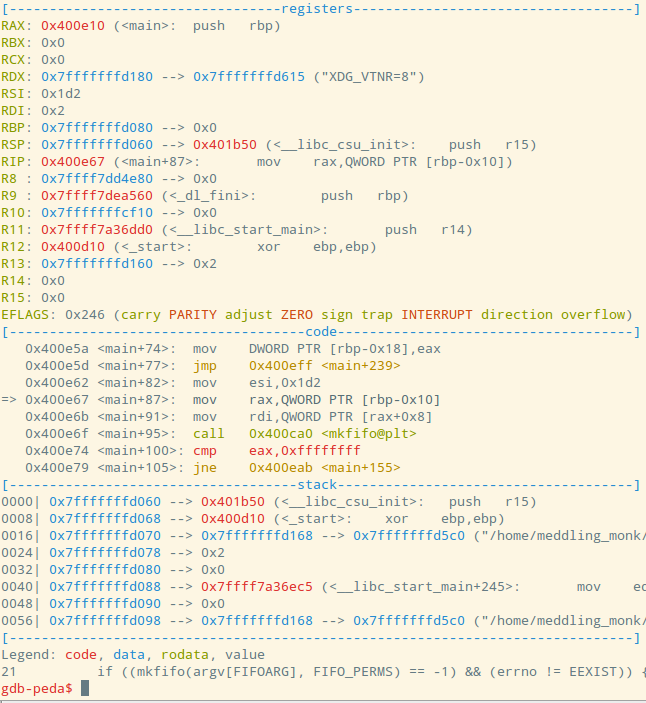
\includegraphics[width=1\linewidth]{./images/4}
	\caption[mkfifo_error_check]{mkfifo() error check}
	\label{fig:4}
\end{figure}
\begin{figure}[H]
	\centering
	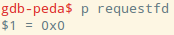
\includegraphics[width=0.3\linewidth]{./images/5}
	\caption[requestfd_val_check_1]{First requestfd value check}
	\label{fig:5}
\end{figure}
\begin{figure}[H]
	\centering
	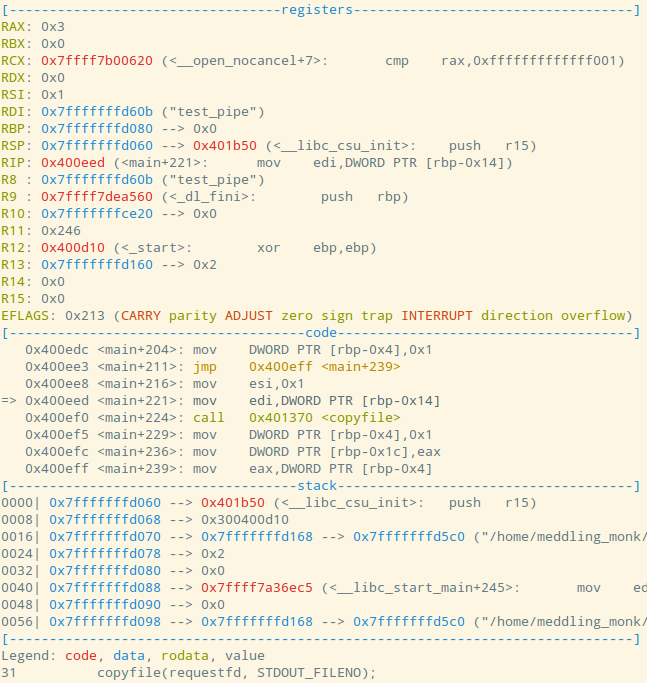
\includegraphics[width=1\linewidth]{./images/6}
	\caption[copyfile]{Copy input from requestfd to the standard out file descriptor}
	\label{fig:6}
\end{figure}
\begin{figure}[H]
	\centering
	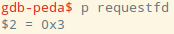
\includegraphics[width=0.3\linewidth]{./images/7}
	\caption[requestfd_val_check_2]{Second requestfd value check}
	\label{fig:7}
\end{figure}
\begin{figure}[H]
	\centering
	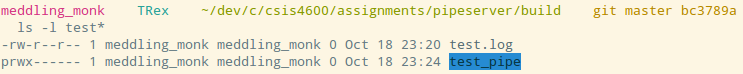
\includegraphics[width=1\linewidth]{./images/8}
	\caption[created_files_listing]{Listing of files created by pipeserver process}
	\label{fig:8}
\end{figure}
\begin{figure}[H]
	\centering
	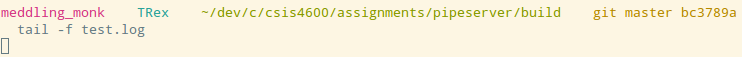
\includegraphics[width=1\linewidth]{./images/9}
	\caption[tailf]{Monitoring test.log with tail -f}
	\label{fig:9}
\end{figure}
\begin{figure}[H]
	\centering
	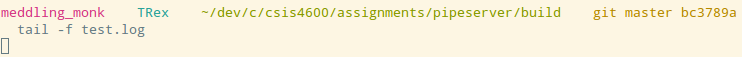
\includegraphics[width=1\linewidth]{./images/9}
	\caption[tailf]{Monitoring test.log with tail -f}
	\label{fig:9}
\end{figure}
\begin{figure}[H]
	\centering
	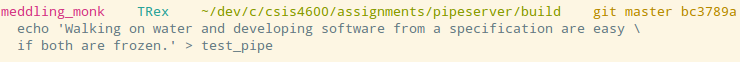
\includegraphics[width=1\linewidth]{./images/10}
	\caption[text_redirection]{Redirection of echoed text to the pipe}
	\label{fig:10}
\end{figure}
\begin{figure}[H]
	\centering
	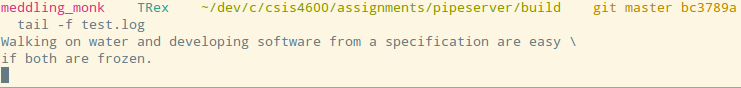
\includegraphics[width=1\linewidth]{./images/11}
	\caption[tail_pipe_follow]{Results from tail's pipe follow}
	\label{fig:11}
\end{figure}
\begin{figure}[H]
	\centering
	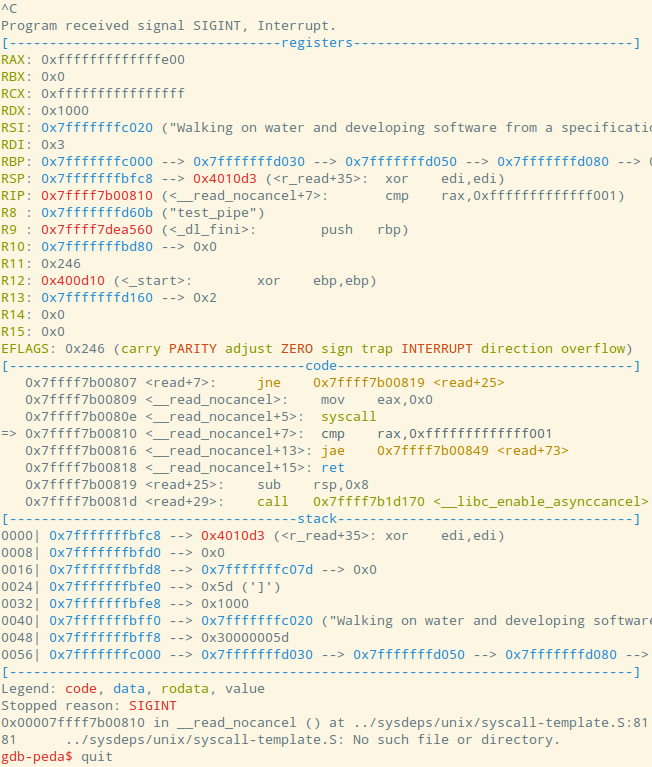
\includegraphics[width=1\linewidth]{./images/12}
	\caption[sigint]{End the pipeserver process}
	\label{fig:12}
\end{figure}
\end{document}